%TCIDATA{LaTeXparent=0,0,relatorio.tex}
\chapter{Fundamentos\label{chap:FundamentacaoMatematica}}

% Resumo opcional. Comentar se não usar.
\resumodocapitulo{Este capítulo apresenta equações básicas do sistema que se deseja validar, assim como informações sobre a bancada laboratorial e também sobre a programação do CLP.}

\section{Equações Governantes}

Estruturas submarinas tais como os \textit{risers} são esbeltas e tem um alto módulo de cisalhamento. Portanto, a simplificação de Euler-Bernoulli para vigas é utilizada para propósitos de modelagem. O deslocamento de interesse é o horizontal e o \textit{riser} está sob a ação de forças hidrodinâmicas externas e de tração. A equação diferencial parcial para a variável deslocamento, $\Upsilon$, é dada por \begin{align}
	m_s \frac{\partial^2 \Upsilon}{\partial t^2} &= -E J	\frac{\partial^4 \Upsilon}{\partial z^4} + \frac{\partial}{\partial z}\left(T(z) \frac{\partial \Upsilon}{\partial z}\right) + F_n(z,t),
\end{align} na qual $m_s$ é a densidade linear do tubo, $E$ é o módulo de Young e $J$ é o segundo momento de inércia do \textit{riser}. $T(z)$ descreve as forças de tração ao longo do comprimento do \textit{riser}. $F_n(z,t)$ é a força resultante externa \cite{fabricioIFAC}.

As únicas forças externas atuando no \textit{riser} são hidrodinâmicas, exceto nas extremidades do topo e do fundo, nas quais forças de reação seguem condições de contorno. A equação de Morison descreve a força externa resultante: \begin{align}
	F_n(z,t) &= -m_f \frac{\partial^2 \Upsilon}{\partial t^2} - \mu\left|\frac{\partial \Upsilon}{\partial t}\right|\frac{\partial \Upsilon}{\partial t},
\end{align} na qual $m_f$ é a massa do fluido adicionado e $\mu$ é o coeficiente de arrasto. Seja $m = m_s + m_f$ 

\section{Controle}
\paragraph{} Técnicas de controle simples devem ser introduzidas de forma a se compreender o objetivo deste trabalho, que é do posicionamento do \textit{riser} por meio de controle em malha fechada. Primeiramente, apresenta-se o controle em malha aberta, cujo diagrama pode ser observado na Figura \ref{mabertatikz}. A variável $r = r(t)$ é a referência do sistema. Neste tipo de controle, a saída não é realimentada na entrada. Desta forma, este tipo de controle não requer sensores, pois somente dá uma referência de entrada que a planta deve seguir. Caso haja erros para seguir a trajetória, eles não poderão ser compensados e é um controle mais recomendado quando o sistema é preciso e há pouca ou nenhuma perturbação. No entanto, este não é o caso do \textit{riser}, pois o movimento das águas no leito oceânico perturba o tubo, causando erros na posição final desejada.

\tikzstyle{block} = [draw, fill=blue!20, rectangle, 
minimum height=3em, minimum width=6em]
\tikzstyle{sum} = [draw, fill=blue!20, circle, node distance=1cm]
\tikzstyle{input} = [coordinate]
\tikzstyle{output} = [coordinate]
\tikzstyle{pinstyle} = [pin edge={to-,thin,black}]

\begin{figure}[!ht]
	\centering
	% The block diagram code is probably more verbose than necessary
	\begin{tikzpicture}[auto, node distance=2cm,>=latex']
	% We start by placing the blocks
	\node [input, name=input] {};
	\node [block, right of=input] (controller) {Controlador};
	\node [block, right of=controller, pin={[pinstyle]above:Perturbações},
	node distance=3cm] (system) {Planta};
	% We draw an edge between the controller and system block to 
	% calculate the coordinate u. We need it to place the measurement block. 
	\draw [->] (controller) -- node[name=u] {$u$} (system);
	\node [output, right of=system] (output) {};
	
	% Once the nodes are placed, connecting them is easy. 
	\draw [draw,->] (input) -- node {$r$} (controller);
	\draw [->] (system) -- node [name=y] {$y$}(output); 
	\end{tikzpicture}
	\caption{Malha aberta de controle\label{mabertatikz}}
\end{figure}

\paragraph{} Uma forma de se compensar as perturbações do ambiente é realimentando a saída na entrada, calculando a diferença entre a referência e o valor medido. Assim, um valor de erro $e = e(t)$ é obtido e o sistema calcula o sinal $u$ conforme o erro evolui. A Figura \ref{mfechadatikz} mostra um esquema básico deste sistema.

\paragraph{} O controle malha aberta foi anteriormente verificado na referência \cite{redytton}.
\begin{figure}[!ht]
\centering
% The block diagram code is probably more verbose than necessary
\begin{tikzpicture}[auto, node distance=2cm,>=latex']
% We start by placing the blocks
\node [input, name=input] {};
\node [sum, right of=input] (sum) {};
\node [block, right of=sum] (controller) {Controlador};
\node [block, right of=controller, pin={[pinstyle]above:Perturbações},
node distance=3cm] (system) {Planta};
% We draw an edge between the controller and system block to 
% calculate the coordinate u. We need it to place the measurement block. 
\draw [->] (controller) -- node[name=u] {$u$} (system);
\node [output, right of=system] (output) {};
\node [block, below of=u] (measurements) {Medição};

% Once the nodes are placed, connecting them is easy. 
\draw [draw,->] (input) -- node {$r$} (sum);
\draw [->] (sum) -- node {$e$} (controller);
\draw [->] (system) -- node [name=y] {$y$}(output);
\draw [->] (y) |- (measurements);
\draw [->] (measurements) -| node[pos=0.99] {$-$} 
node [near end] {$y_m$} (sum);
\end{tikzpicture}
\caption{Malha fechada de controle\label{mfechadatikz}}
\end{figure}

\section{Bancada}
A bancada da ponte rolante presente no Laboratório de Automação e Controle está esquematizada na Figura \ref{bancadaEsquematico}. Serão detalhados os componentes desta bancada, de modo a se entender o papel de cada um deles. Observe que no esquemático falta a câmera, que é um sensor que fica de frente para a bancada. 

\begin{figure}[hbt]
\centering
  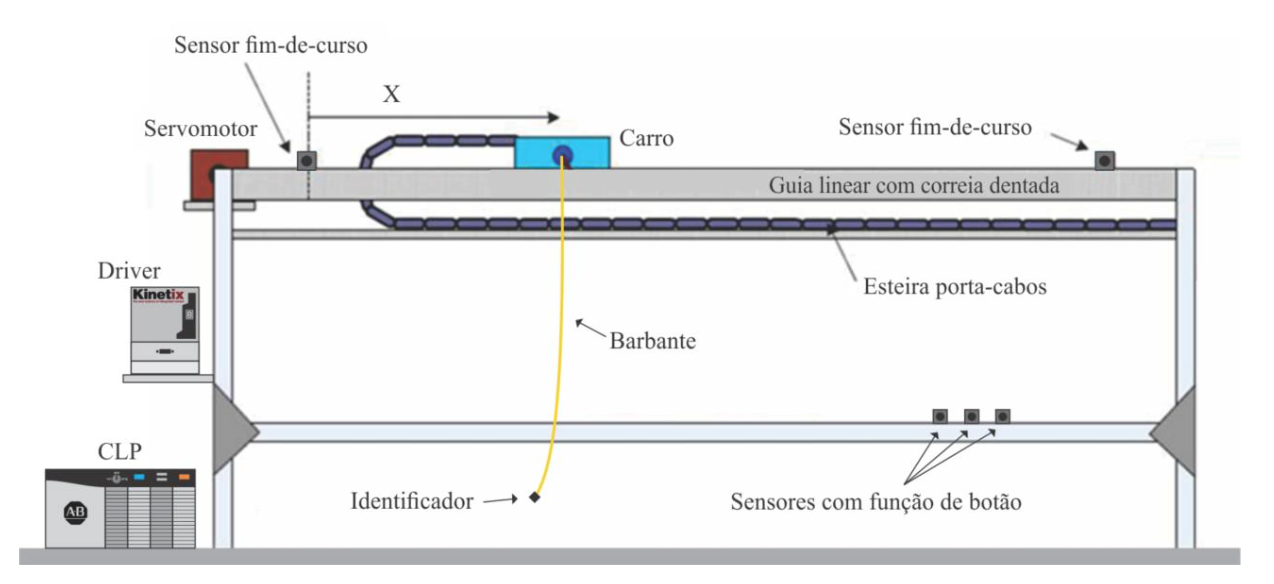
\includegraphics[width=0.8\textwidth]{figs/fundamentos/bancadaEsquematico}
  \caption{Esquemático da Bancada Utilizada para o Experimento \cite{redytton}\label{bancadaEsquematico}}
\end{figure}

\subsection{Controlador Lógico-Programável}
\begin{figure}[!ht]
  \centering
    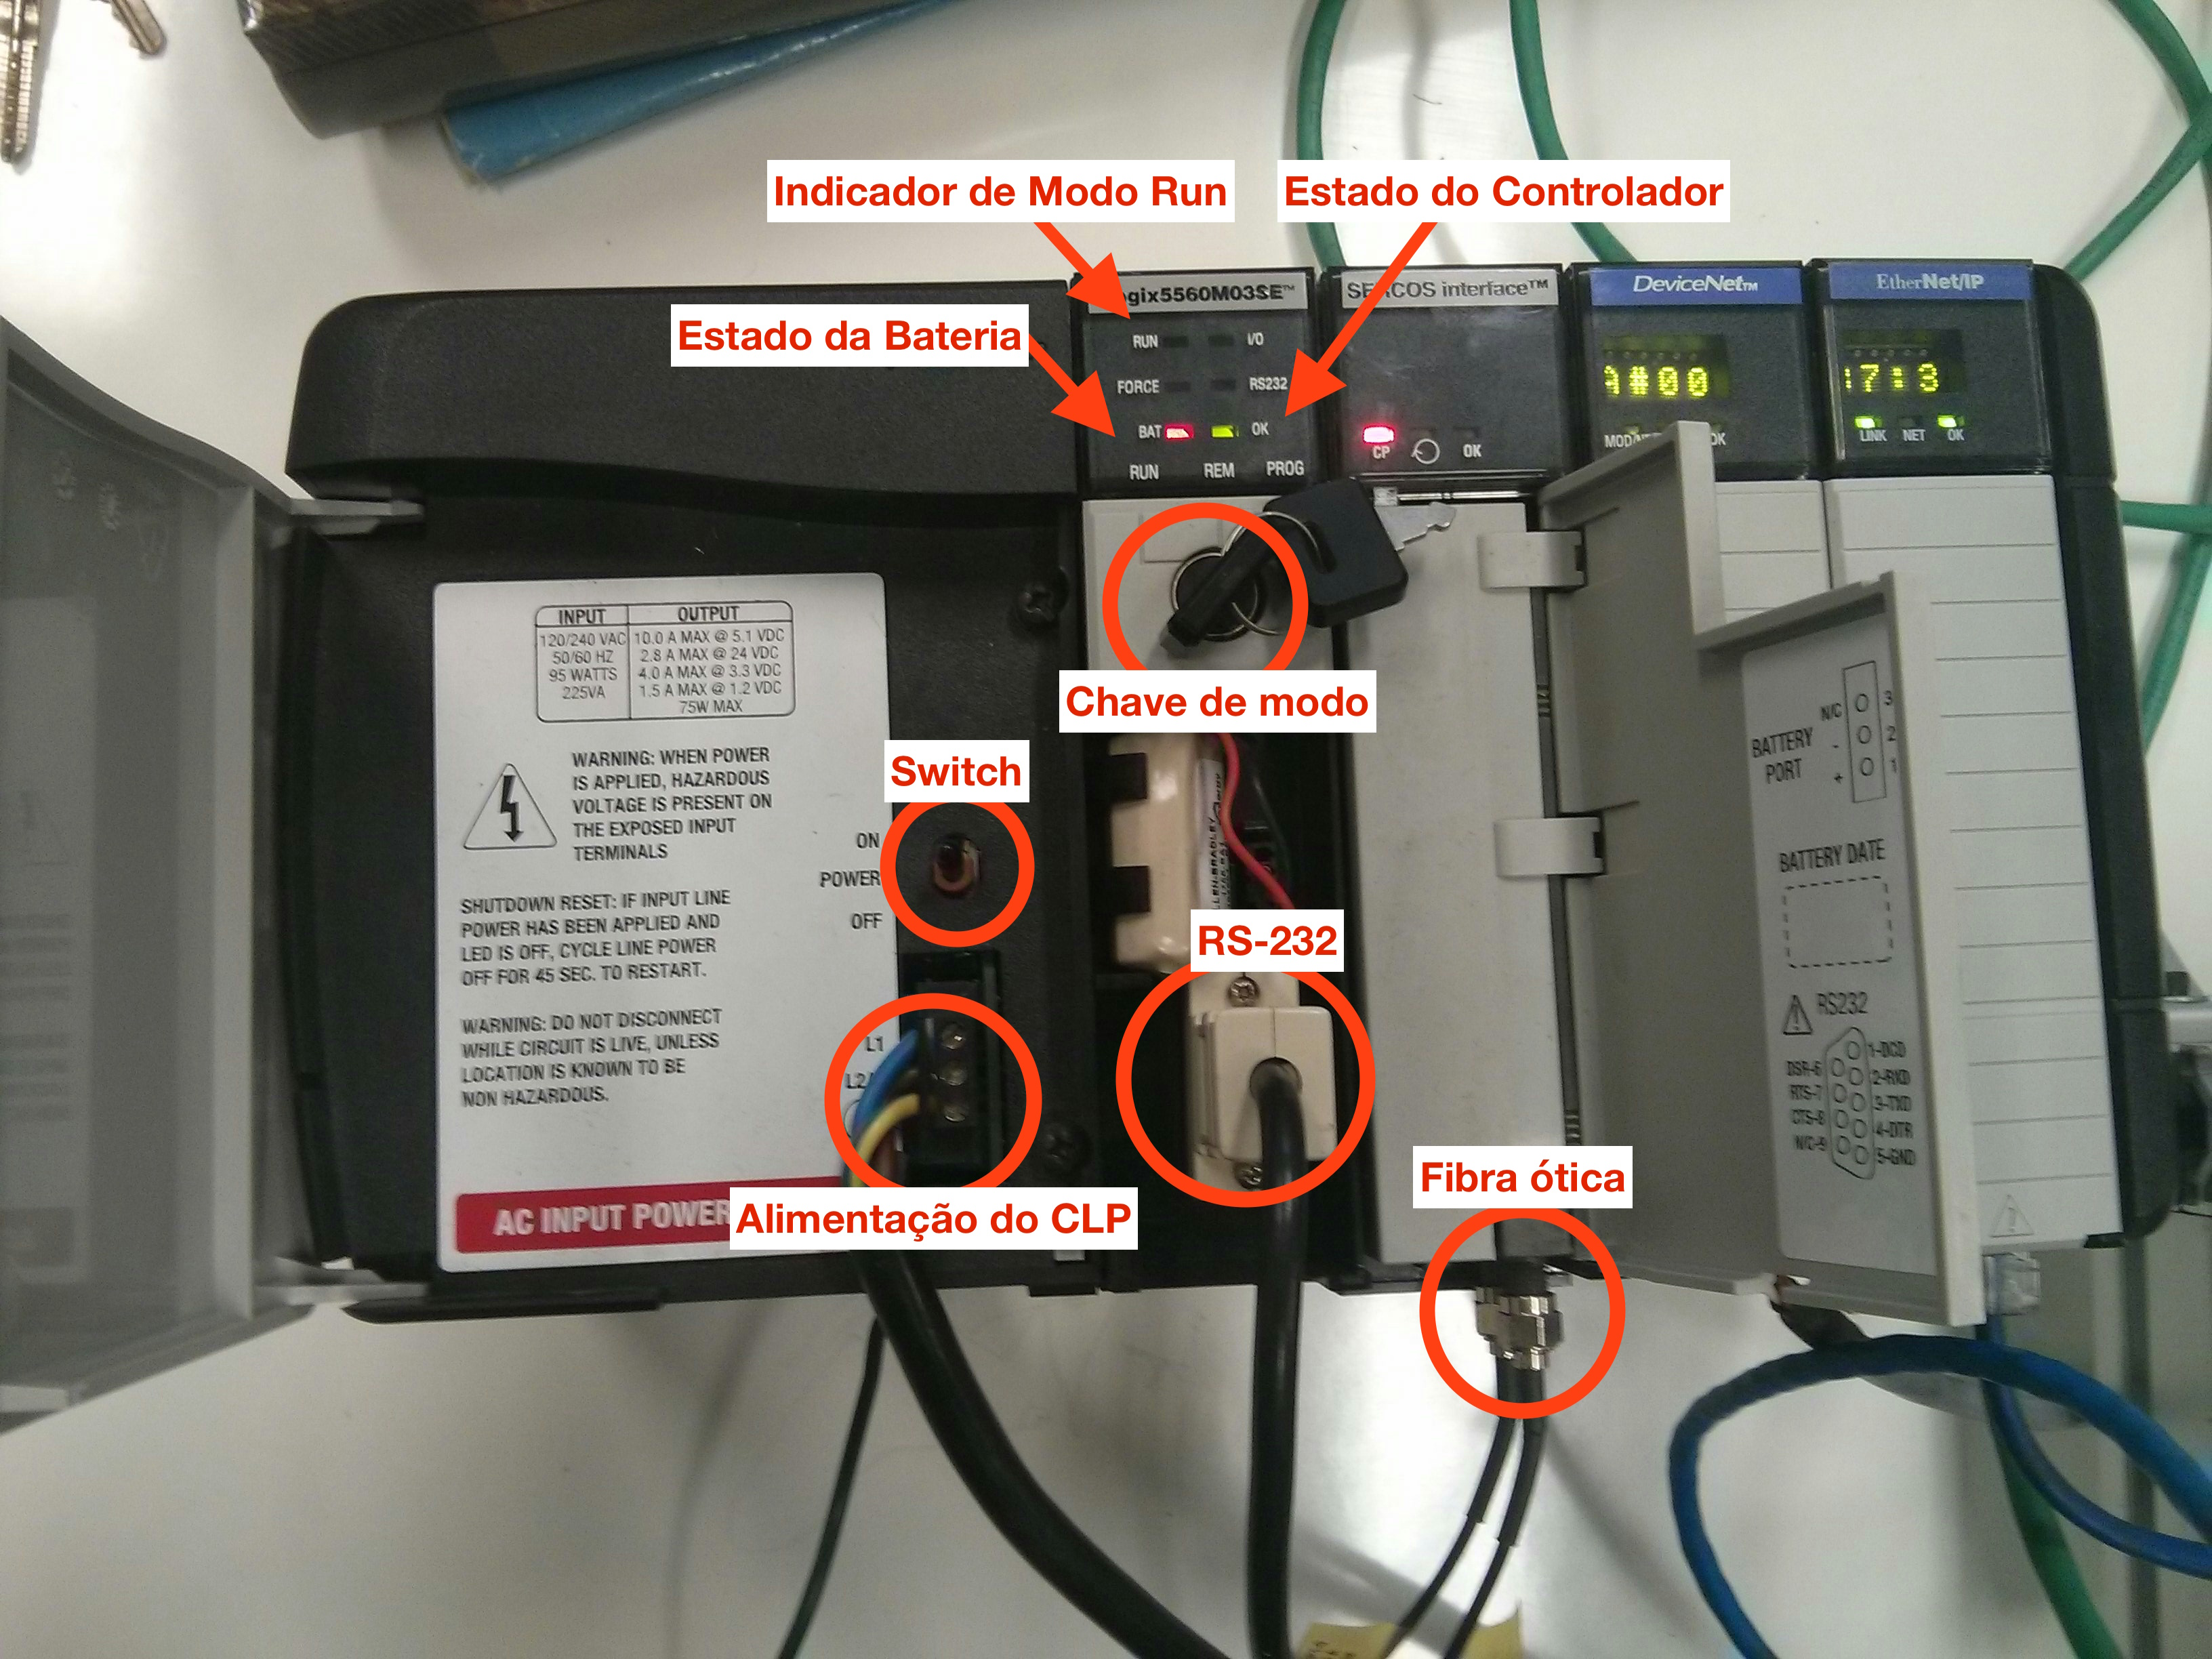
\includegraphics[width=0.8\textwidth]{figs/fundamentos/CLP.jpg}
    \caption{CLP com identificação de elementos\label{CLPcomentado}}
\end{figure}

\paragraph{} O controlador lógico-programável (CLP - ver Figura \ref{CLPcomentado}) é a espinha dorsal da bancada. Ele é responsável por executar os comandos de controle sobre todos os elementos que estão conectados a ele. A programação do CLP é realizada via computador, mas, uma vez feito o \textit{download} do programa ao CLP, a execução ocorre independentemente do computador, contato que o CLP esteja em modo de execução.
\paragraph{} O CLP utilizado é fabricado pela \textit{Allen Bradley}, modelo Logix5560M03SE. Tal modelo possui memória lógica e de dados de 750 KiB, e memória de \textit{I/O} de 494 KiB. Há quatro módulos no \textit{chassis} do controlador:
\begin{itemize}
  \item O próprio controlador;
  \item \textit{SERCOS Interface};
  \item DeviceNET;
  \item EtherNet/IP.
\end{itemize}
\paragraph{} Cada um desses módulos será apresentado posteriormente com mais detalhes. Além dos módulos, o controlador ainda possui um \textit{switch} liga/desliga presente no \textit{chassis}. No módulo Logix, há uma chave responsável por alterar o modo de funcionamento do mesmo. As posições possíveis dessa chave são:
\begin{itemize}
  \item RUN;
  \item REM;
  \item PROG;
\end{itemize}
\paragraph{} Na prática, o modo REM se divide em dois modos: REM RUN e REM PROG. A maneira de se diferenciar os dois é observar, no módulo Logix, o estado do LED indicador de modo RUN quando a chave estiver na posição REM.
\paragraph{} No modo RUN, o controlador apenas roda o programa presente em sua memória; não há qualquer comunicação remota. No modo PROG, o controlador não roda nenhum programa; ele apenas pode receber um novo código. Nos modos REM, há a comunicação com o computador, permitindo verificar valores de variáveis de interesse e alterar, se necessário, o programa a ser rodado pelo controlador. O programa presente no controlador, em modo REM, só roda o código se estiver no modo REM RUN; se for necessário atualizar o programa, o modo deve ser o REM PROG.

\subsection{SERCOS Interface}

Sercos é um barramento digital de automação que interconecta controladores, \textit{drives}, dispositivos de entrada/saída e atuadores para máquinas e sistemas controlados numericamente. Foi projetado para comunicação serial de alta velocidade de dados em sistemas de tempo real por meio de fibra ótica (Sercos I \& II) ou um cabo Ethernet Industrial (Sercos III). Sercos é um padrão internacional \cite{sercos}.

Num sistema Sercos, todas as malhas que contém servomotores são normalmente fechadas no \textit{drive}. Isto reduz a carga computacional no CLP, permitindo-o sincronizar mais eixos do que conseguiria caso contrário. Além disso, fechar a malha dos servomotores com o \textit{driver} ajuda a reduzir o efeito do atraso de transporte entre o controle de movimento e o \textit{driver} \cite{sercos}.

Nesta bancada, o CLP deve se comunicar com o servomotor (MPL-A310F-SJ22AA) através do \textit{drive} Kinetix (2094-AC05MP5), de forma a movimentar o carrinho segundo uma trajetória planejada ou segundo uma lei de controle em malha fechada executando no CLP. Essa comunicação se dá por um par de fibras óticas full-duplex, conforme se observa na Figura \ref{CLPcomentado}, o que caracteriza uma rede Sercos I ou II.

\subsection{Line Interface Module 2094-AL09}

Este módulo não apareceu no esquemático da Figura \ref{bancadaEsquematico}, mas ele tem a função essencial de interfacear a rede trifásica com o servo \textit{drive}, permitindo o acionamento do motor. Na Figura \ref{LineInterfaceModule}, se observa que há três conjuntos de disjuntores nesse módulo: CB1 \textendash{} liga ou desliga a rede trifásica do \textit{drive}  \textendash{}, CB2 \textendash{} fornece tensão monofásica ao servo \textit{drive} \textendash{} e CB3 \textendash{} liga as duas fontes de tensão DC de 24V \textendash{}, responsáveis pelas entradas e saídas digitais do módulo e alimentação do freio do motor \cite{redytton}.

\begin{figure}[!ht]
  \centering
    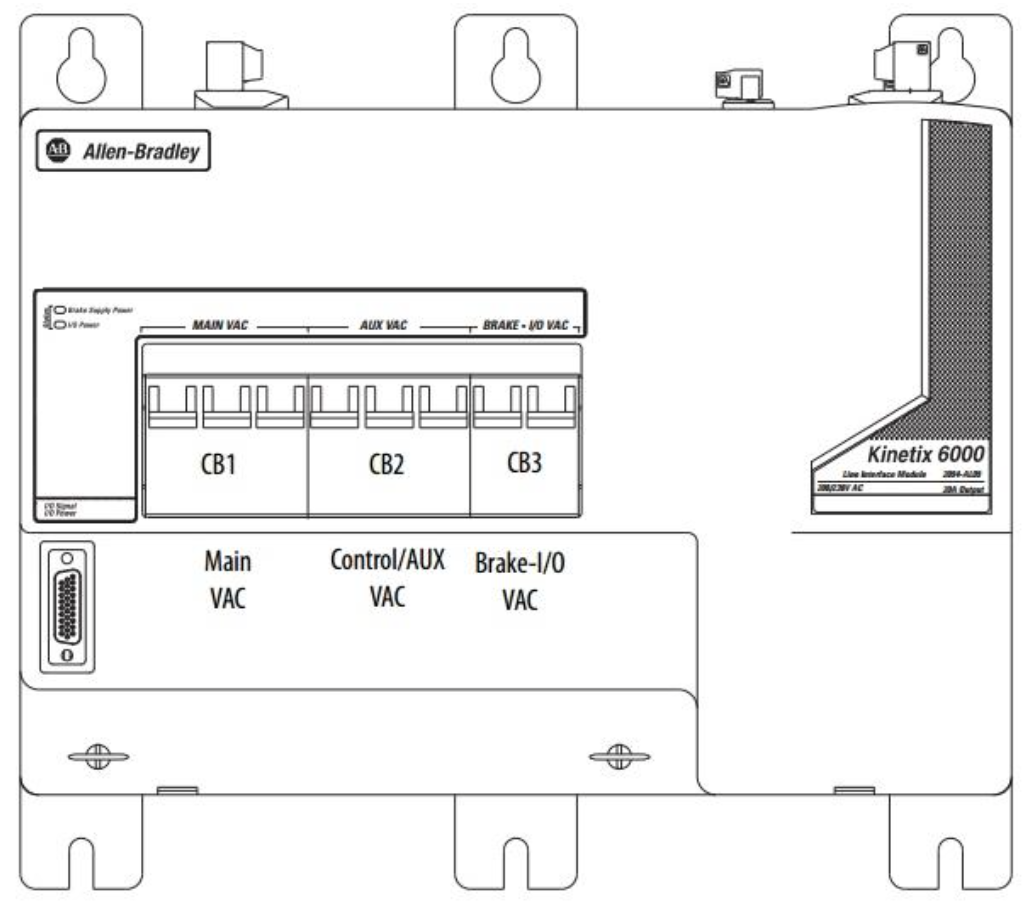
\includegraphics[width=0.7\textwidth]{figs/fundamentos/LineInterfaceModule}
    \caption{Line Interface Module modelo 2094-AL09 da Allen Bradley \cite{redytton}\label{LineInterfaceModule}}
\end{figure}

\subsection{Drive Kinetix 6000 da Allen Bradley}

Por meio da Interface Sercos, o CLP comanda o drive que então fornece potência ao motor. O drive controla o servomotor por meio de pulsos PWM. A Figura \ref{kinetix6000} apresenta um Drive Kinetix 6000 da Allen Bradley similar ao utilizado no laboratório. Mais detalhes sobre o funcionamento do drive estão disponíveis em \cite{redytton} e \cite{kinetix6000usermanual}.

\begin{figure}[!ht]
  \centering
    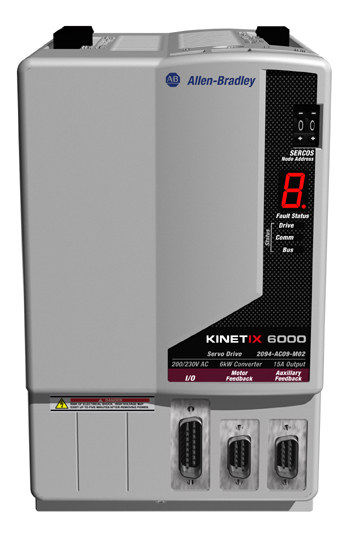
\includegraphics[width=0.3\textwidth]{figs/fundamentos/kinetix6000.jpg}
    \caption{Drive Kinetix 6000 da Allen Bradley\label{kinetix6000}}
\end{figure}

\subsection{Servomotor}

Um servomotor é um atuador rotatório que permite controle preciso da posição angular. O motor consiste de um motor acoplado a um sensor para a realimentação de posição/velocidade. Também é necessário um drive servo para completar o sistema. O \textit{drive} usa o sensor de realimentação para controlar precisamente a posição angular do motor, ou seja, é uma operação em malha fechada. Assim, usando servomotores em malha fechada, tem-se uma alternativa de alto desempenho aos motores de passo e de indução \cite{defServoMotores}.

O servomotor MPL-A310F-SJ22AA da \textit{Allen-Bradley} foi utilizado e está representado na Figura \ref{servomotor}. O mesmo é composto por um motor indutivo de tensão nominal $230V_{\mathrm{ac}}$ e um encoder do tipo StegmanHiperface, que mede posição de forma absoluta e velocidade de forma incremental \cite{redytton}.

\begin{figure}[!ht]
  \centering
    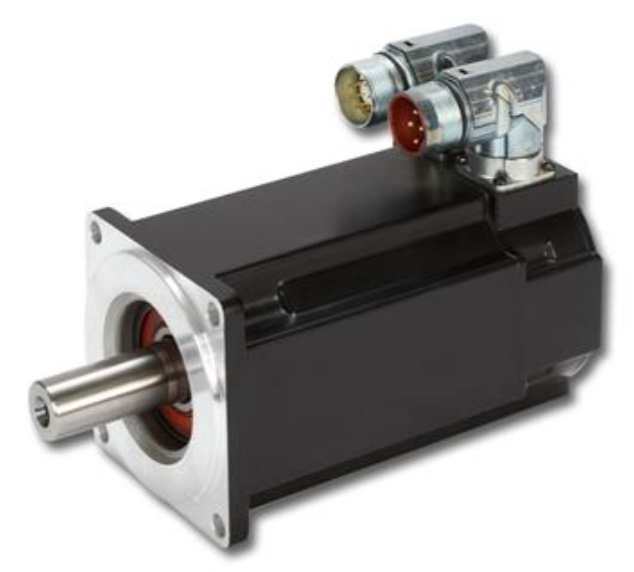
\includegraphics[width=0.3\textwidth]{figs/fundamentos/servomotor}
    \caption{Servomotor modelo MPL-A310F-SJ22AA\label{servomotor}}
\end{figure}

\subsection{Sensores indutivos}
Os sensores indutivos são elementos detectores de presença, particularmente de objetos metálicos. Eles funcionam através da variação de campo magnético ocasionada pela presença do objeto a ser identificado. Tal variação de campo magnético provoca uma variação de corrente dentro do sensor, alterando seu estado.

Na presente bancada, há 6 sensores indutivos da família 871TM, similares ao da Figura \ref{sensorIndutivo}, fabricados pela \textit{Allen-Bradley}. Eles são alimentados com tensão de 24 V, que está dentro dos limites padrão. São sensores feitos de aço, adaptados a ambientes industriais.

\begin{figure}[!ht]
  \centering
    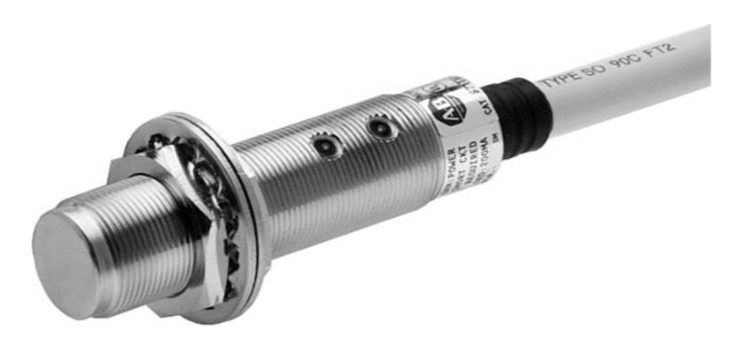
\includegraphics[width=0.3\textwidth]{figs/fundamentos/sensorIndutivo}
    \caption{Sensor indutivo 871T-R8B18 \cite{redytton}\label{sensorIndutivo}}
\end{figure}

A importância desses sensores é enorme. O motivo é que a câmera às vezes falha para obter a posição atual e tem um limite de frequência devido ao processamento interno que ela tem de realizar. Com os sensores indutivos, tem-se um processamento rápido para identificar se o motor está na região próxima dos limites. Assim, a rotina de segurança que trava o motor depende diretamente desses sensores indutivos.

\subsection{Câmera PresencePlus}

A câmera PresencePlus P4 GEO da Banner Engineering foi utilizada no projeto - veja Figura \ref{cameraBanner}. Esta câmera é um sensor robusto utilizado em ambientes industriais com fácil utilização. Sua programação é feita em software próprio da Banner e é visual.

Dentre as capacidades da câmera, nota-se que ela pode capturar até 24 imagens por segundo. No entanto, além da captura das imagens há o processamento das imagens, que pode ser feito na própria câmera ou em um módulo externo da própria Banner, que também consome certo tempo. O programa utilizado no projeto está disponível no Anexo ...

%TODO colocar imagens do programa da câmera
%TODO colocar programa da banner no github e colocar link para ele

\begin{figure}[!ht]
  \centering
    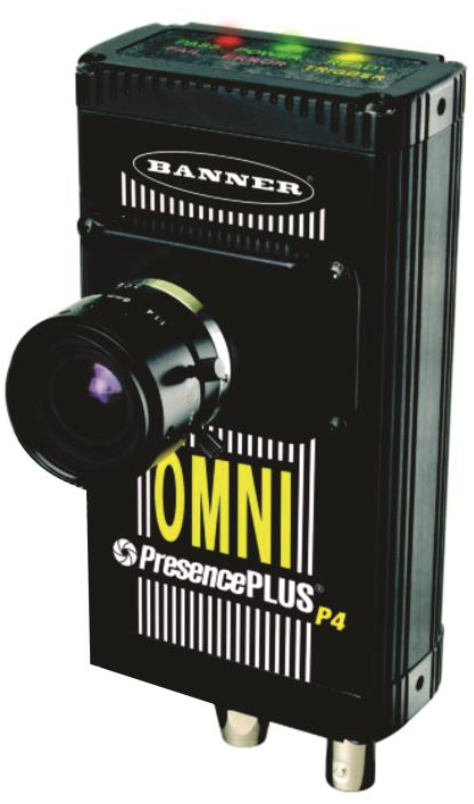
\includegraphics[width=0.3\textwidth]{figs/fundamentos/camera}
    \caption{Câmera da Banner Engineering utilizada no projeto \cite{redytton}\label{cameraBanner}}
\end{figure}

\section{Redes Utilizadas}
\subsection{DeviceNET}
\paragraph{}DeviceNET é um protocolo de baixo nível da camada de aplicação, voltado a ambientes industriais. É responsável pela interconexão de dispositivos visando ao compartilhamento de dados. Foi desenvolvido pela \textit{Allen-Bradley}, em cima da tecnologia CAN (\textit{Control Area Networking}) desenvolvida pela \textit{Bosch}. Tal rede suporta comunicação entre dispositivos de baixo nível, como sensores e atuadores, e dispositivos de alto nível, como o computador e o CLP. 
\paragraph{}O DeviceNET é uma combinação entre a camada física disponibilizada pelo CAN e um protocolo industrial, o CIP (\textit{Common Industrial Protocol}), que rege as redes industriais em geral. Permite uma rápida configuração entre dispositivos a \textit{byte}, suportanto tanto dispositivos analógicos quanto digitais. Permite velocidades de transmissão de até 500 kbps, sendo bem mais lenta que uma rede Ethernet.
\paragraph{}No experimento, a rede DeviceNET é utilizada para a conexão entre o CLP e os sensores indutivos presentes na planta.\cite{redytton} Devido à flexibilidade dos sensores e da rede, suas informações podem ser trabalhadas tanto no modo analógico quanto no modo digital. Para fins de detecção de fim-de-curso, entretanto, o modo utilizado é o digital, uma vez que não será preciso determinar a distância entre sensor e carrinho; apenas é necessário verificar se o carrinho está na área de detecção do sensor. O módulo responsável pelo gerenciamento da rede DeviceNET é o 1756-DNB.

\begin{comment}
https://en.wikipedia.org/wiki/DeviceNet
http://ab.rockwellautomation.com/Networks-and-Communications/DeviceNet-Network
http://www.rtaautomation.com/technologies/devicenet/
https://www.odva.org/Portals/0/Library/Publications_Numbered/PUB00122R1_CIP_Brochure_ENGLISH.pdf
\end{comment}

\subsection{Ethernet-IP}
\paragraph{}A rede Ethernet-IP, desenvolvida em meados dos anos 1990, é um tipo de rede Ethernet voltada ao ambiente industrial, seguindo o CIP, assim como o DeviceNET. É uma rede robusta, organizada segundo o modelo OSI de 7 camadas, que permite conexão com dispositivos conectados a redes Ethernet padrão; permite a passagem de dados via pacotes TCP ou UDP; é indicada em aplicações que exigem uma transferência rápida de dados (principalmente, em aplicações de tempo real).
\paragraph{}O uso da rede Ethernet-IP é vantajoso no sentido de que permite a conexão entre vários nós ligados entre si, o que não é possível com o RS-232, por exemplo. Porém, devido ao próprio funcionamento da rede, fica mais difícil obter os dados, pois, ao contrário de uma entrada serial, é necessário lidar com toda uma estrutura baseada no TCP/IP, por exemplo. Além disso, como o Ethernet exige um tamanho mínimo de \textit{frame} para transmissão de dados de cerca de 64 \textit{bytes}, a eficiência da transmissão pode ser afetada.
\paragraph{}No presente experimento, a rede Ethernet-IP é utilizada para receber dados de inspeção da câmera, notadamente a posição da bola de isopor presa ao barbante. Além disso, ela é utilizada na transferência de programas entre o computador e o CLP (através do módulo Ethernet 1756-ENBT/A), uma vez que ela provê uma comunicação mais rápida do que o RS-232.

\begin{comment}
https://en.wikipedia.org/wiki/Industrial_Ethernet
https://en.wikipedia.org/wiki/EtherNet/IP
https://www.odva.org/Technology-Standards/EtherNet-IP/Overview
http://www.rtaautomation.com/technologies/ethernetip/
http://www.rockwellautomation.com/global/products-technologies/integrated-architecture/ethernet-ip.page
http://www.rtaautomation.com/technologies/ethernetip/
\end{comment}

\section{Programação do CLP}
\subsection{Visão geral}
\paragraph{}Programação, em termos gerais, é aplicada na resolução de problemas. Em particular, a programação de CLPs busca resolver, no âmbito industrial, problemas relacionados à automação de processos. Essa resolução de problemas segue uma metodologia, de forma a se direcionar o projeto. Antes de se proceder a programação, faz-se necessário seguir os seguintes passos \cite{rockwellAutomation}:
\begin{enumerate}
  \item Descrição do problema;
  \item Detalhamentos e melhoria do processo;
  \item Especificação dos atuadores e sensores da planta;
  \item Elaboração do algoritmo;
  \item Representação gráfica do algoritmo, quando aplicável;
  \item Esquema funcional, quando aplicável;
  \item Seleção dos módulos do controlador;
  \item Programação, utilizando linguagens suportadas.
\end{enumerate}
\paragraph{}Ao se programar o CLP, deve-se ter em conta que o controlador executa sempre três ciclos:
\begin{enumerate}
  \item \textit{Scan} de Entrada: Ciclo em que o controlador recebe todos os dados de seus módulos de entrada;
  \item \textit{Scan} do Programa: Ciclo em que o controlador processa as entradas recebidas e gera as saídas;
  \item \textit{Scan} de Saída: Ciclo em que o controlador envia os dados de saída para os módulos de saída.
\end{enumerate}
\paragraph{}Para o presente experimento, entre as várias linguagens disponíveis para CLPs, foram selecionadas duas: uma linguagem gráfica, o \textbf{\textit{ladder}}, e uma linguagem textual, o \textbf{texto estruturado}.

\subsection{Linguagem \textit{ladder}}
\subsubsection{Introdução ao \textit{ladder}}
\paragraph{}A linguagem \textit{ladder} é uma linguagem de programação gráfica, e uma das primeiras a ser utilizada na programação de CLPs. Seu nome vem do inglês \textit{ladder}, que significa escada; nome dado em razão dos programas, ao serem feitos, assumirem a forma de uma escada, e lidos de cima para baixo (movimento de descida). Essa linguagem foi estruturada de forma a ter uma simbologia semelhante à de um diagrama de conexão de relés, que eram utilizados em indústrias antes do CLP.
\paragraph{}Todo programa \textit{ladder} possui duas linhas verticais e, entre elas, uma ou mais linhas horizontais nas quais são especificados os comportamentos do programa. A linguagem possui várias instruções, em sua maioria comuns entre diferentes tipos de CLP. A tabela \ref{ladder1} mostra as principais instruções utilizadas em \textit{ladder}, utilizando a sintaxe presente no \textit{software} RSLogix5000:

\begin{table}[!ht]
  \centering
  \caption{Principais instruções \textit{ladder} \label{ladder1}}
  \begin{tabular}{|c|c|c|}
    \hline
    Desenho da Instrução & Nome da Instrução & Descrição \\ \hline
    -( )- & OTE & Atualiza variável de acordo com a condição da linha \\ \hline
    -(L)- & OTL & Liga variável se a linha for alimentada \\ \hline
    -(U)- & OTU & Desliga variável se a linha for alimentada \\ \hline
    -[ ]- & XIC & Examina se a variável está ligada \\ \hline
    -[/]- & XIO & Examina se a variável está desligada \\ \hline
  \end{tabular}
\end{table}

\subsubsection{Instruções específicas}
\paragraph{}O presente experimento utiliza, em sua programação, não apenas elementos básicos da linguagem \textit{ladder}. A presença do servomotor exige uma lógica e entradas que não são booleanas, ou seja, que não poderm ser tratadas pelos operadores descritos na tabela \ref{ladder1}. Portanto, faz-se necessário o uso de novas instruções, diretamente relacionadas com o movimento do atuador. Tais instruções são conhecidas, dentro do RSLogix5000, como \textit{Motion Control Instructions}, ou instruções de controle de movimento. A tabela \ref{ladder2} mostra as instruções desse tipo utilizadas no experimento:

\begin{table}[!ht]
  \centering
  \caption{Principais instruções de controle de movimento em \textit{ladder} \label{ladder2}}
  \begin{tabularx}{\textwidth}{|>{\bfseries}l|l|X|}
    \hline
    Nome da Instrução & Sigla & Função \\ \hline
    \textit{Motion Servo On} & MSO & Inicializa o servomotor, travando a esteira. \\ \hline
    \textit{Motion Axis Jog} & MAJ & Envia comandos de velocidade e sentido de rotação ao motor, executando sua movimentação. \\ \hline
    \textit{Motion Axis Stop} & MAS & Interrompe a movimentação do motor; a esteira permanece travada. \\ \hline
    \textit{Motion Servo Off} & MSF & 
    Desativa o servomotor, destravando a esteira e permitindo a movimentação manual do carrinho.\\ \hline
  \end{tabularx}
\end{table}

\paragraph{}As funções descritas pela tabela \ref{ladder2} lidam com outros tipos de variáveis, como números reais, para a velocidade do motor, e até mesmo estruturas que o \textit{software} RSLogix cria para armazenar informações sobre os eixos e o controle feito pelas instruções. Tais parâmetros podem ser alterados dentro dos blocos das funções. A figura \ref{motionladder1} mostra um exemplo de tais instruções:

\begin{figure}[!ht]
  \centering
    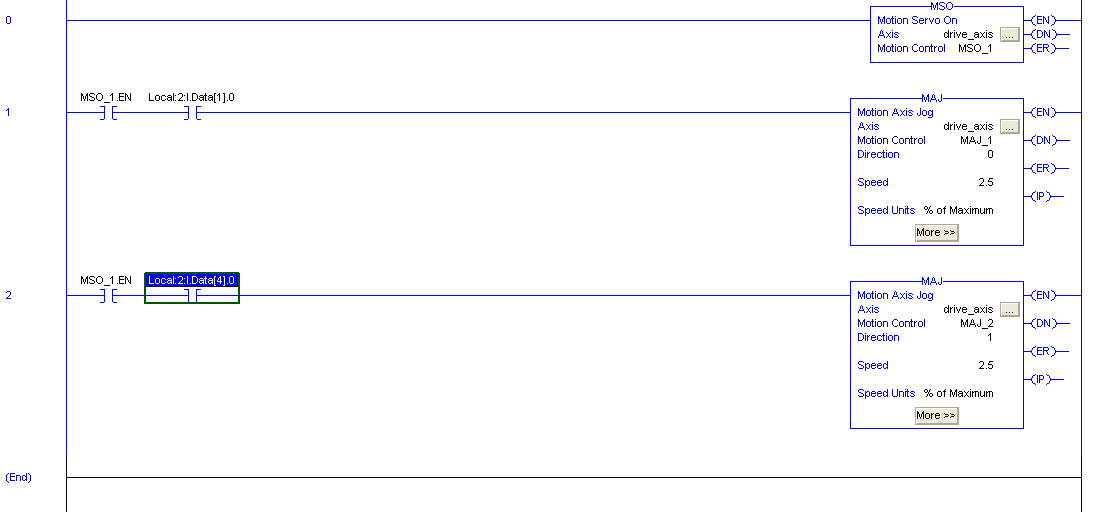
\includegraphics[width=0.6\textwidth]{figs/fundamentos/motionladder}
    \caption{Exemplo de programa \textit{ladder} com instruções de movimentação.\label{motionladder1}}
\end{figure}

\subsection{Texto Estruturado}
\subsubsection{Visão geral do texto estruturado}
\paragraph{}Além de \textit{ladder}, que é uma linguagem gráfica, o CLP utilizado no experimento também suporta uma linguagem puramente textual, o texto estruturado. Essa linguagem é uma linguagem sequencial, que lembra muito linguagens como BASIC, C ou Pascal. Cada comando é executado em sequência, salvo em caso de desvios (estruturas do tipo \textit{if-then-else}) ou repetições (\textit{loops}, estruturas do tipo \textit{while}).
\paragraph{}Em relação ao \textit{ladder}, o texto estruturado possui vantagens e desvantagens. A principal vantagem é o fato do texto estruturado se assemelhar às linguagens de programação mais utilizadas; isso torna tal linguagem de fácil aprendizado. Além disso, por ser texto, programas escritos dessa forma podem ser gerados com auxílio de outros programas, codificados em linguagens como \textit{Python}, por exemplo. Tal característica torna a alteração de vários parâmetros por vez extremamente simples, pois a mudança de código no programa auxiliar para lidar com as mudanças do controlador programado é mínima. Porém, uma desvantagem do texto em relação ao \textit{ladder} reside nas funções de movimentação, uma vez que, ao contrário do \textit{ladder}, o texto estruturado não dá uma indicação clara associando um valor e a variável que ele representa, além da ordem dos parâmetros. Isso torna o uso de funções como MAJ (vide tabela \ref{ladder2}) um pouco mais complicada em texto. Cabe ao programador ponderar as vantagens e desvantagens das duas linguagens ao desenvolver o programa para o CLP, de forma a garantir os melhores resultados.
\subsubsection{Instruções de movimentação do motor para o texto estruturado}
\paragraph{}Assim como o \textit{ladder}, o texto estruturado permite o uso das funções descritas na tabela \ref{ladder2}. A sintaxe de uso dessas funções lembra muito a sintaxe da linguagem C, com o nome da função e uma lista de parâmetros válidos separados por vírgulas. A seguir, um exemplo de uso:
 
\begin{lstlisting}
  MSO(drive_axis,MSO_1);

  speed[0] := 0.0;
  dataInitialized := 1;
\end{lstlisting}

\paragraph{}Nota-se que o código apresentado, a menos da operação de atribuição, possui uma sintaxe muito semelhante à de C. A função MSO acima recebe dois parâmetros, assim como em \textit{ladder}; porém, a única indicação de como os parâmetros se comportam é a ordem com que eles são colocados; no caso de MSO, o 1º parâmetro é o eixo que será inicializado, e o 2º parâmetro é uma \textit{tag} que guarda as informações de controle executadas por MSO.


\section{Parâmetros para gerar trajetórias}

\paragraph{}Fabrício et al \cite{fabricioIFAC} desenvolveram um método para gerar trajetórias \textit{offline} (controle malha aberta) assim como \textit{online} (controle malha fechada). Para se utilizar do método, é necessário ter parâmetros do sistema. Se se fosse simular ou controlar o sistema real, utilizariam-se os dados da Tabela \ref{escalaReal}, conforme referência \cite{redytton}.

\begin{table}[!ht]
\centering
\caption{Dados para simulação em escala real\label{escalaReal} \cite{redytton}}
	\begin{tabular}{|c|c|}
	\hline
		\multicolumn{2}{|c|}{\textbf{Dados do Riser}}\\ \hline
		Diâmetro externo & $0.55\mathrm{m}$\\ \hline
		Diâmetro interno & $0.5\mathrm{m}$ \\ \hline
		Comprimento & $2000\mathrm{m}$ \\ \hline
		Módulo de Elasticidade & $200 \mathrm{GPa}$\\ \hline
		Densidade &  $7860\mathrm{kg}/\mathrm{m}^3$\\ \hline
		\multicolumn{2}{|c|}{\textbf{Dados do fluido (Água)}}\\ \hline
		Densidade do fluido &  $1000\mathrm{kg}/\mathrm{m}^3$\\ \hline
		Viscosidade dinâmica & $10^3 \mathrm{Pa}\cdot \mathrm{s}$ \\ \hline
	\end{tabular}
\end{table}

\paragraph{}Como é importante se validar o sistema, mas nem sempre isso é possível em escala real devido ao altíssimo custo e aos riscos envolvidos, é necessário um conjunto equivalente de parâmetros tais que permita validar o sistema em escala laboratorial. O \textit{riser} é representado por um barbante e a água é trocada pelo ar. Uma massa na ponta foi adicionada e os dados resultantes estão na Tabela \ref{escalaLaboratorial}.

\begin{table}[!ht]
\centering
\caption{Dados para simulação em escala laboratorial\label{escalaLaboratorial}}
	\begin{tabular}{|c|c|}
	\hline
		\multicolumn{2}{|c|}{\textbf{Dados da Massa na Ponta - Isopor}} \\ \hline
		Diâmetro Externo & $30.6\mathrm{mm}$\\ \hline
		Densidade & $10\mathrm{kg}/\mathrm{m}^3$ \\ \hline
		\multicolumn{2}{|c|}{\textbf{Dados do Riser (Barbante)}}\\ \hline
		Diâmetro externo & $2\mathrm{mm}$\\ \hline
		Diâmetro interno & $0\mathrm{mm}$ \\ \hline
		Comprimento & $82\mathrm{cm}$ \\ \hline
		Módulo de Elasticidade & $2.1 \mathrm{MPa}$\\ \hline
		Densidade &  $191\mathrm{kg}/\mathrm{m}^3$\\ \hline
		\multicolumn{2}{|c|}{\textbf{Dados do fluido (Ar)}}\\ \hline
		Densidade do fluido &  $1.2754\mathrm{kg}/\mathrm{m}^3$\\ \hline
		Viscosidade dinâmica & $17.2\cdot 10^6 \mathrm{Pa}\cdot \mathrm{s}$ \\ \hline
	\end{tabular}
\end{table}
